\حصہء{سوالات}
\موٹا{قطبی محددی جوڑیاں}\\
\ابتدا{سوال}\شناخت{سوال_مخروط_قطبی_کارتیسی_الف}
کون سی محددی جوڑیاں ایک ہی نقطہ کو ظاہر کرتی ہیں۔\\
\begin{multicols}{4}
\begin{enumerate}[a.]
\item
$(3,0)$
\item
$(-3,0)$
\item
$(2,\tfrac{2\pi}{3})$
\item
$(2,\tfrac{7\pi}{3})$
\item
$(-3,\pi)$
\item
$(2,\tfrac{\pi}{3})$
\item
$(-3,2\pi)$
\item
$(-2,-\tfrac{\pi}{3})$
\end{enumerate}
\end{multicols}
جواب:\quad
ا اور ہ؛  ب اور ز؛ ج اور ح؛ د اور و 
\انتہا{سوال}
%===================
\ابتدا{سوال}
کون سی محددی جوڑیاں ایک ہی نقطہ کو ظاہر کرتی ہیں۔\\
\begin{multicols}{4}
\begin{enumerate}[a.]
\item
$(-2,\tfrac{\pi}{3})$
\item
$(2,-\tfrac{\pi}{3})$
\item
$(r,\theta)$
\item
$(r,\theta+\pi)$
\item
$(-r,\theta)$
\item
$(2,-\tfrac{2\pi}{3})$
\item
$(-r,\theta+\pi)$
\item
$(-2,\tfrac{2\pi}{3})$
\end{enumerate}
\end{multicols}
\انتہا{سوال}
%===================
\ابتدا{سوال}\شناخت{سوال_مخروط_قطبی_نقطے}
درج ذیل قطبی محدد میں دیے گئے نقطے ترسیم کریں۔ ان نقطوں کے تمام قطبی محدد تلاش کریں۔ 
\begin{multicols}{4}
\begin{enumerate}[a.]
\item
$(2,\tfrac{\pi}{2})$
\item
$(2,0)$
\item
$(-2,\tfrac{\pi}{2})$
\item
$(-2,0)$
\end{enumerate}
\end{multicols}
جواب:\quad
شکل \حوالہ{شکل_سوال_مخروط_قطبی_نقطے}\\
(ا) \عددی{(2,\tfrac{\pi}{2}+2n\pi)} اور \عددی{(-2,\tfrac{\pi}{2}+(2n+1)\pi)} جہاں \عددی{n} عدد صحیح ہے۔\\
(ب) \عددی{(2,2n\pi)} اور \عددی{(-2,(2n+1)\pi)} جہاں \عددی{n} عدد صحیح ہے۔\\
(ج) \عددی{(2,\tfrac{3\pi}{2}+2n\pi)} اور \عددی{(-2,\tfrac{3\pi}{2}+(2n+1)\pi)} جہاں \عددی{n} عدد صحیح ہے۔\\
(د) \عددی{(2,(2n+1)\pi)} اور \عددی{(-2,2n\pi)} جہاں \عددی{n} عدد صحیح ہے۔
\انتہا{سوال}
%=================
\ابتدا{سوال}
درج ذیل قطبی محدد میں دیے گئے نقطے ترسیم کریں۔ ان نقطوں کے تمام قطبی محدد تلاش کریں۔ 
\begin{multicols}{4}
\begin{enumerate}[a.]
\item
$(3,\tfrac{\pi}{4})$
\item
$(-3,\tfrac{\pi}{4})$
\item
$(3,-\tfrac{\pi}{4})$
\item
$(-3,-\tfrac{\pi}{4})$
\end{enumerate}
\end{multicols}
\انتہا{سوال}
%=================
\موٹا{قطبی سے کارتیسی محدد}\\
\ابتدا{سوال}
ان نقطوں کے کارتیسی محدد معلوم کریں جنہیں سوال \حوالہ{سوال_مخروط_قطبی_کارتیسی_الف} میں پیش کیا گیا ہے۔\\
جواب:\quad
(ا) \عددی{(3,0)}، (ب) \عددی{(-3,0)}، (ج) \عددی{(-1,\sqrt{3})}، (د) \عددی{(1,\sqrt{3})}، (ہ) \عددی{(3,0)}، (و) \عددی{(1,\sqrt{3})}، (ز) \عددی{(-3,0)}، (ح) \عددی{(-1,\sqrt{3})}
\انتہا{سوال}
%==================
\ابتدا{سوال}
درج ذیل نقطے قطبی محدد میں دیے گئے ہیں۔ ان کی کارتیسی محدد تلاش کریں۔
\begin{multicols}{4}
\begin{enumerate}[a.]
\item
$(\sqrt{2},\tfrac{\pi}{4})$
\item
$(1,0)$
\item
$(0,\tfrac{\pi}{2})$
\item
$(-\sqrt{2},\tfrac{\pi}{4})$
\item
$(-3,\tfrac{5\pi}{6})$
\item
$(5,\tan^{-1}(\tfrac{4}{3}))$
\item
$(-1,7\pi)$
\item
$(2\sqrt{3},\tfrac{2\pi}{3})$
\end{enumerate}
\end{multicols}
\انتہا{سوال}
%======================
\موٹا{قطبی مساوات اور عدم مساوات کی ترسیم}\\
سوال \حوالہ{سوال_مخروط_عدم_مساوات_الف} تا سوال \حوالہ{سوال_مخروط_عدم_مساوات_ب} میں دیے مساوات اور عدم مساوات کو مطمئن کرنے والے نقطوں کے سلسلہ کو ترسیم کریں۔ 

\ابتدا{سوال}\شناخت{سوال_مخروط_عدم_مساوات_الف}
$r=2$\\
جواب:\quad 
شکل \حوالہ{شکل_سوال_مخروط_عدم_مساوات_الف}
\انتہا{سوال}
%======================
\ابتدا{سوال}
$0\le r\le 2$
\انتہا{سوال}
%======================
\ابتدا{سوال}
$r\ge 1$\\
جواب:\quad 
شکل \حوالہ{شکل_سوال_مخروط_قطبی_نقطے_پ}
\انتہا{سوال}
%======================
\ابتدا{سوال}
$1\le rle 2$
\انتہا{سوال}
%======================
\ابتدا{سوال}
$0\le \theta\le \tfrac{\pi}{6},\quad r\ge 0$\\
جواب:\quad 
شکل \حوالہ{شکل_سوال_مخروط_قطبی_نقطے_ت}
\انتہا{سوال}
%======================
\ابتدا{سوال}
$\theta=\tfrac{2\pi}{3},\quad r\le -2$
\انتہا{سوال}
%======================
\ابتدا{سوال}
$\theta=\tfrac{\pi}{3},\quad -1\le r\le 3$\\
جواب:\quad 
شکل \حوالہ{شکل_سوال_مخروط_قطبی_نقطے_ٹ}
\انتہا{سوال}
%======================
\ابتدا{سوال}
$\theta=\tfrac{11\pi}{4},\quad r\ge -1$
\انتہا{سوال}
%======================
\ابتدا{سوال}
$\theta=\tfrac{\pi}{2},\quad r\ge 0$\\
جواب:\quad 
شکل \حوالہ{شکل_سوال_مخروط_قطبی_نقطے_ث}
\انتہا{سوال}
%======================
\ابتدا{سوال}
$\theta=\tfrac{\pi}{2},\quad r\le 0$
\انتہا{سوال}
%======================
\ابتدا{سوال}
$0\le \theta\le \pi,\quad r=1$\\
جواب:\quad 
شکل \حوالہ{شکل_سوال_مخروط_قطبی_نقطے_ج}
\انتہا{سوال}
%======================
\ابتدا{سوال}
$0\le \theta\le \pi,\quad r=-1$
\انتہا{سوال}
%======================
\ابتدا{سوال}
$\tfrac{\pi}{4}\le \theta \le \tfrac{3\pi}{4},\quad 0\le r\le 1$\\
جواب:\quad 
شکل \حوالہ{شکل_سوال_مخروط_قطبی_نقطے_چ}
\انتہا{سوال}
%======================
\ابتدا{سوال}
$-\tfrac{\pi}{4}\le \theta \le \tfrac{\pi}{4},\quad -1\le r\le 1$
\انتہا{سوال}
%======================
\ابتدا{سوال}
$-\tfrac{\pi}{2}\le \theta \le \tfrac{\pi}{2},\quad 1\le r\le 2$\\
جواب:\quad 
شکل \حوالہ{شکل_سوال_مخروط_قطبی_نقطے_ح}
\انتہا{سوال}
%======================
\ابتدا{سوال}\شناخت{سوال_مخروط_عدم_مساوات_ب}
$0\le \theta \le \tfrac{\pi}{2},\quad 1\le \abs{r}\le 2$
\انتہا{سوال}
%======================
\begin{figure}
\centering
\begin{minipage}{0.22\textwidth}
\centering
\begin{tikzpicture}[font=\scriptsize]
\pgfmathsetmacro{\k}{pi/2}
\begin{axis}[clip=false,width=4cm, axis lines=middle,xlabel={$x$},ylabel={$y$},enlargelimits=true,xtick={\empty},ytick={\empty}, xlabel style={at={(current axis.right of origin)},anchor=west},ylabel style={at={(current axis.above origin)},anchor=south}]
\addplot[]plot coordinates {(-2,0)}node[circ]{}node[below]{$(-2,0)$};
\addplot[]plot coordinates {(2,0)}node[circ]{}node[below]{$(2,0)$};
\addplot[]plot coordinates {(0,-2)}node[circ]{}node[right]{$(-2,\tfrac{\pi}{2})$};
\addplot[]plot coordinates {(0,2)}node[circ]{}node[right]{$(2,\tfrac{\pi}{2})$};
\end{axis}
\end{tikzpicture}
\caption{}
\label{شکل_سوال_مخروط_قطبی_نقطے}
\end{minipage}\hfill
\begin{minipage}{0.22\textwidth}
\centering
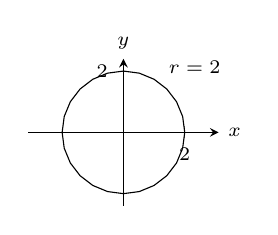
\begin{tikzpicture}[font=\scriptsize,declare function={f(\x)=2*cos(\x);g(\x)=2*sin(\x);}]
\pgfmathsetmacro{\k}{360}
\begin{axis}[axis equal,clip=false,width=4cm, axis lines=middle,xlabel={$x$},ylabel={$y$},enlargelimits=true,xtick={2},ytick={2}, xlabel style={at={(current axis.right of origin)},anchor=west},ylabel style={at={(current axis.above origin)},anchor=south}]
\addplot[domain=0:\k]({f(x)},{g(x)})node[pos=0.15,above right]{$r=2$};
\end{axis}
\end{tikzpicture}
\caption{}
\label{شکل_سوال_مخروط_عدم_مساوات_الف}
\end{minipage}\hfill
\begin{minipage}{0.22\textwidth}
\centering
\begin{tikzpicture}[font=\scriptsize,declare function={f(\x)=cos(\x);g(\x)=sin(\x);}]
\pgfmathsetmacro{\k}{1.5}
\begin{axis}[axis on top,axis equal,clip=false,width=4cm, axis lines=middle,xlabel={$x$},ylabel={$y$},enlargelimits=true,xtick={1},ytick={\empty}, xlabel style={at={(current axis.right of origin)},anchor=west},ylabel style={at={(current axis.above origin)},anchor=south}]
\addplot[fill=lgray,draw=none]plot coordinates {(-\k,-\k)(\k,-\k)(\k,\k)(-\k,\k)(-\k,-\k)};
\addplot[fill=white,domain=0:360]({f(x)},{g(x)});
\addplot[] plot coordinates {(1.25,0.25)}node[pin=45:{$r\ge 1$}]{};
\end{axis}
\end{tikzpicture}
\caption{}
\label{شکل_سوال_مخروط_قطبی_نقطے_پ}
\end{minipage}
\end{figure}
%==================
\begin{figure}
\centering
\begin{minipage}{0.22\textwidth}
\centering
\begin{tikzpicture}[font=\scriptsize]
\pgfmathsetmacro{\kx}{cos(30)}
\pgfmathsetmacro{\ky}{sin(30)}
\begin{axis}[axis on top,clip=false,width=4cm, axis lines=middle,xlabel={$x$},ylabel={$y$},xtick={\empty},ytick={\empty}, xlabel style={at={(current axis.right of origin)},anchor=west},ylabel style={at={(current axis.above origin)},anchor=south}]
\addplot[-latex,name path=a]plot coordinates {(0,0) (\kx,\ky)}node[pos=0.7,left]{$\begin{aligned}  0\le &\theta\le \tfrac{\pi}{6} \\ r&\ge 0 \end{aligned}$};
\path[name path=xaxis](axis cs:0,0)--(axis cs:\kx,0);
\addplot[lgray] fill between [of=a and xaxis];
\end{axis}
\end{tikzpicture}
\caption{}
\label{شکل_سوال_مخروط_قطبی_نقطے_ت}
\end{minipage}\hfill
\begin{minipage}{0.22\textwidth}
\centering
\begin{tikzpicture}[font=\scriptsize,declare function={f(\x)=0.6*cos(\x);g(\x)=0.6*sin(\x);}]
\pgfmathsetmacro{\kxa}{-1*cos(60)}
\pgfmathsetmacro{\kya}{-1*sin(60)}
\pgfmathsetmacro{\kxb}{3*cos(60)}
\pgfmathsetmacro{\kyb}{3*sin(60)}
\begin{axis}[axis on top,clip=false,width=4cm, axis lines=middle,xlabel={$x$},ylabel={$y$},xtick={-1,2},ytick={-1,3}, xlabel style={at={(current axis.right of origin)},anchor=west},ylabel style={at={(current axis.above origin)},anchor=south},enlargelimits=true,xmin=-1.1,xmax=2.2,ymax=3.2]
\addplot[]plot coordinates {(\kxa,\kya)(\kxb,\kyb)}node[pos=0,circ]{}node[pos=1,circ]{}node[pos=1,above]{$\begin{aligned} \theta&=\tfrac{\pi}{3}\\ -1&\le r\le 3 \end{aligned}$};
\addplot[-stealth,domain=0:60]({f(x)},{g(x)})node[pos=0.75,right]{$\theta$};
\end{axis}
\end{tikzpicture}
\caption{}
\label{شکل_سوال_مخروط_قطبی_نقطے_ٹ}
\end{minipage}\hfill
\begin{minipage}{0.22\textwidth}
\centering
\begin{tikzpicture}[font=\scriptsize,declare function={f(\x)=0.6*cos(\x);g(\x)=0.6*sin(\x);}]
\pgfmathsetmacro{\kxa}{-1*cos(60)}
\pgfmathsetmacro{\kya}{-1*sin(60)}
\pgfmathsetmacro{\kxb}{3*cos(60)}
\pgfmathsetmacro{\kyb}{3*sin(60)}
\begin{axis}[axis on top,clip=false,width=4cm, axis lines=middle,xlabel={$x$},ylabel={$y$},xtick={\empty},ytick={\empty}, xlabel style={at={(current axis.right of origin)},anchor=west},ylabel style={at={(current axis.above origin)},anchor=south},enlargelimits=true,ymax=1.25]
\addplot[-stealth,thick]plot coordinates {(0,0)(0,1)}node[pos=0,circ]{}node[pos=0.5,right]{$\begin{aligned} \theta&=\tfrac{\pi}{2}\\ r&\ge 0\end{aligned}$};
\end{axis}
\end{tikzpicture}
\caption{}
\label{شکل_سوال_مخروط_قطبی_نقطے_ث}
\end{minipage}
\end{figure}
%==============================
\begin{figure}
\centering
\begin{minipage}{0.22\textwidth}
\centering
\begin{tikzpicture}[font=\scriptsize,declare function={f(\x)=cos(\x);g(\x)=sin(\x);}]
\begin{axis}[axis equal,axis on top,clip=false,width=4cm, axis lines=middle,xlabel={$x$},ylabel={$y$},xtick={1},ytick={\empty}, xlabel style={at={(current axis.right of origin)},anchor=west},ylabel style={at={(current axis.above origin)},anchor=south},enlargelimits=true]
\addplot[domain=0:180]({f(x)},{g(x)})node[pos=0.25,above right]{$\begin{aligned}r&=1\\ 0&\le \theta\le \pi   \end{aligned}$};
\end{axis}
\end{tikzpicture}
\caption{}
\label{شکل_سوال_مخروط_قطبی_نقطے_ج}
\end{minipage}\hfill
\begin{minipage}{0.22\textwidth}
\centering
\begin{tikzpicture}[font=\scriptsize,declare function={f(\x)=cos(\x);g(\x)=sin(\x);}]
\begin{axis}[axis equal,axis on top,clip=false,width=4cm, axis lines=middle,xlabel={$x$},ylabel={$y$},xtick={\empty},ytick={1}, xlabel style={at={(current axis.right of origin)},anchor=west},ylabel style={at={(current axis.above origin)},anchor=south},enlargelimits=true]
\addplot[name path=c,domain=45:135]({f(x)},{g(x)})node[pos=0.25,above right]{$\begin{aligned}\tfrac{\pi}{4}&\le\theta\le\tfrac{3\pi}{4}\\  0&\le r\le 1  \end{aligned}$};
\addplot[name path=b]plot coordinates {({cos(135)},{sin(135)})(0,0) ({cos(45)},{sin(45)})};
\addplot[lgray]fill between[of=b and c];
\end{axis}
\end{tikzpicture}
\caption{}
\label{شکل_سوال_مخروط_قطبی_نقطے_چ}
\end{minipage}\hfill
\begin{minipage}{0.22\textwidth}
\centering
\begin{tikzpicture}[font=\scriptsize,declare function={f(\x)=cos(\x);g(\x)=sin(\x);}]
\begin{axis}[axis equal,axis on top,clip=false,width=4cm, axis lines=middle,xlabel={$x$},ylabel={$y$},xtick={1,2},xticklabels={\llap{$1$},\rlap{$2$}},ytick={1,2}, xlabel style={at={(current axis.right of origin)},anchor=west},ylabel style={at={(current axis.above origin)},anchor=south},enlargelimits=true]
\addplot[name path=b,domain=-90:90]({2*f(x)},{2*g(x)})node[pos=0.75,above right]{$\begin{aligned}-\tfrac{\pi}{2}&\le\theta\le\tfrac{\pi}{2}\\  1&\le r\le 2  \end{aligned}$};
\addplot[name path=c,domain=-90:90]({f(x)},{g(x)});
\addplot[lgray]fill between[of=b and c];
\end{axis}
\end{tikzpicture}
\caption{}
\label{شکل_سوال_مخروط_قطبی_نقطے_ح}
\end{minipage}
\end{figure}
\موٹا{قطبی سے کارتیسی مساوات}\\
سوال \حوالہ{سوال_مخروط_قطبی_سے_کارتیسی_الف} تا سوال \حوالہ{سوال_مخروط_قطبی_سے_کارتیسی_ب} میں مطابقتی کارتیسی مساوات دریافت کریں۔ اس کے بعد ترسیم کو پہچانئے۔

\ابتدا{سوال}\شناخت{سوال_مخروط_قطبی_سے_کارتیسی_الف}
$r\cos\theta=2$
\انتہا{سوال}
%===================
\ابتدا{سوال}
$r\sin\theta=-1$
\انتہا{سوال}
%===================
\ابتدا{سوال}
$r\sin\theta=0$
\انتہا{سوال}
%===================
\ابتدا{سوال}
$r\cos\theta=0$
\انتہا{سوال}
%===================
\ابتدا{سوال}
$r=4\csc \theta$
\انتہا{سوال}
%===================
\ابتدا{سوال}
$r=-3\sec\theta$
\انتہا{سوال}
%===================
\ابتدا{سوال}
$r\cos\theta+r\sin\theta=1$
\انتہا{سوال}
%===================
\ابتدا{سوال}
$r\sin\theta=r\cos\theta$
\انتہا{سوال}
%===================
\ابتدا{سوال}
$r^2=1$
\انتہا{سوال}
%===================
\ابتدا{سوال}
$r^2=4r\sin\theta$
\انتہا{سوال}
%===================
\ابتدا{سوال}
$r=\tfrac{5}{\sin\theta-2\cos\theta}$
\انتہا{سوال}
%===================
\ابتدا{سوال}
$r^2\sin2\theta=2$
\انتہا{سوال}
%===================
\ابتدا{سوال}
$r=\cot\theta\csc\theta$
\انتہا{سوال}
%===================
\ابتدا{سوال}
$r=4\tan\theta\sec\theta$
\انتہا{سوال}
%===================
\ابتدا{سوال}
$r=\csc\theta e^{r\cos\theta}$
\انتہا{سوال}
%===================
\ابتدا{سوال}
$r\sin\theta=\ln r+\ln\cos\theta$
\انتہا{سوال}
%===================
\ابتدا{سوال}
$r^2+2r^2\cos\theta\sin\theta=1$
\انتہا{سوال}
%===================
\ابتدا{سوال}
$\cos^2\theta=\sin^2\theta$
\انتہا{سوال}
%===================
\ابتدا{سوال}
$r^2=-4r\cos\theta$
\انتہا{سوال}
%===================
\ابتدا{سوال}
$r62=-6r\sin\theta$
\انتہا{سوال}
%===================
\ابتدا{سوال}
$r=8\sin\theta$
\انتہا{سوال}
%===================
\ابتدا{سوال}
$r=3\cos\theta$
\انتہا{سوال}
%===================
\ابتدا{سوال}
$r=2\cos\theta+2\sin\theta$
\انتہا{سوال}
%===================
\ابتدا{سوال}
$r=2\cos\theta-\sin\theta$
\انتہا{سوال}
%===================
\ابتدا{سوال}
$r\sin(\theta+\tfrac{\pi}{6})=2$
\انتہا{سوال}
%===================
\ابتدا{سوال}\شناخت{سوال_مخروط_قطبی_سے_کارتیسی_ب}
$r=r\sin(\tfrac{2\pi}{3}-\theta)=5$
\انتہا{سوال}
%===================

\موٹا{کارتیسی سے قطبی مساوات}\\
سوال \حوالہ{سوال_مخروط_کارتیسی_سے_قطبی_الف} تا سوال \حوالہ{سوال_مخروط_کارتیسی_سے_قطبی_ب} میں کارتیسی مساوات سے قطبی مساوات حاصل کریں۔ 

\ابتدا{سوال}\شناخت{سوال_مخروط_کارتیسی_سے_قطبی_الف}
$x=7$
\انتہا{سوال}
%========================
\ابتدا{سوال}
$y=1$
\انتہا{سوال}
%========================
\ابتدا{سوال}
$x=y$
\انتہا{سوال}
%========================
\ابتدا{سوال}
$x-y=3$
\انتہا{سوال}
%========================
\ابتدا{سوال}
$x^2+y^2=4$
\انتہا{سوال}
%========================
\ابتدا{سوال}
$x^2-y^2=1$
\انتہا{سوال}
%========================
\ابتدا{سوال}
$\tfrac{x^2}{9}+\tfrac{y^2}{4}=1$
\انتہا{سوال}
%========================
\ابتدا{سوال}
$xy=2$
\انتہا{سوال}
%========================
\ابتدا{سوال}
$y^2=4x$
\انتہا{سوال}
%========================
\ابتدا{سوال}
$x^2+xy+y^2=1$
\انتہا{سوال}
%========================
\ابتدا{سوال}
$x^2+(y-2)^2=4$
\انتہا{سوال}
%========================
\ابتدا{سوال}
$(x-5)^2+y^2=25$
\انتہا{سوال}
%========================
\ابتدا{سوال}
$(x-3)^2+(y+1)^2=4$
\انتہا{سوال}
%========================
\ابتدا{سوال}\شناخت{سوال_مخروط_کارتیسی_سے_قطبی_ب}
$(x+2)^2+(y-5)^2=16$
\انتہا{سوال}
%========================

\موٹا{نظریہ اور مثالیں}\\
\ابتدا{سوال}
مبدا کے تمام قطبی محدد تلاش کریں۔
\انتہا{سوال}
%=============
\ابتدا{سوال}\ترچھا{افقی اور انتصابی خط}\\
\begin{enumerate}[a.]
\item
دکھائیں کہ \عددی{xy} مستوی میں ہر انتصابی خط کی قطبی مساوات کو \عددی{r=a\sec\theta} لکھا جا سکتا ہے۔
\item
\عددی{xy} مستوی میں ہر افقی خط کی  قطبی مساوات کس صورت کی ہو گی؟
\end{enumerate}
\انتہا{سوال}
%==================
